\chapter{Konzeptionelles Modell}

	\section{Generisch vs. generativ}
		Zuerst muss entschieden werden, welche Teile des Codes generiert werden k�nnen und bei 
		welchen Teilen ein generativer Ansatz besser ist. Um mit der HsrOrderApp\_S3 als Vorlage m�glichst 
		bald eine lauff�hige HsrOrderApp\_S4 mit generiertem Code zu erhalten, werden wir uns 
		auf die Generierung von Domain Objekt Klassen und Mapper Klassen beschr�nken.

		Die Beschreibungen f�r die Generierung des Codes werden in abstrakten Klassen gemacht.		
		
		Da UnitOfWork, Identity Map und einige Finder Methoden noch generisch implementiert werden,
		ist es n�tig, dass die Domain Objekte von einer gemeinsamen Oberklasse abgeleitet werden.
		Die Klasse \verb~DomainObject~ ist Teil der \textit{STORM} Library. Die abstrakten Klassen m�ssen 
		von dieser abgeleitet werden.
		
		\begin{figure}[hbt]
			\begin{center}
				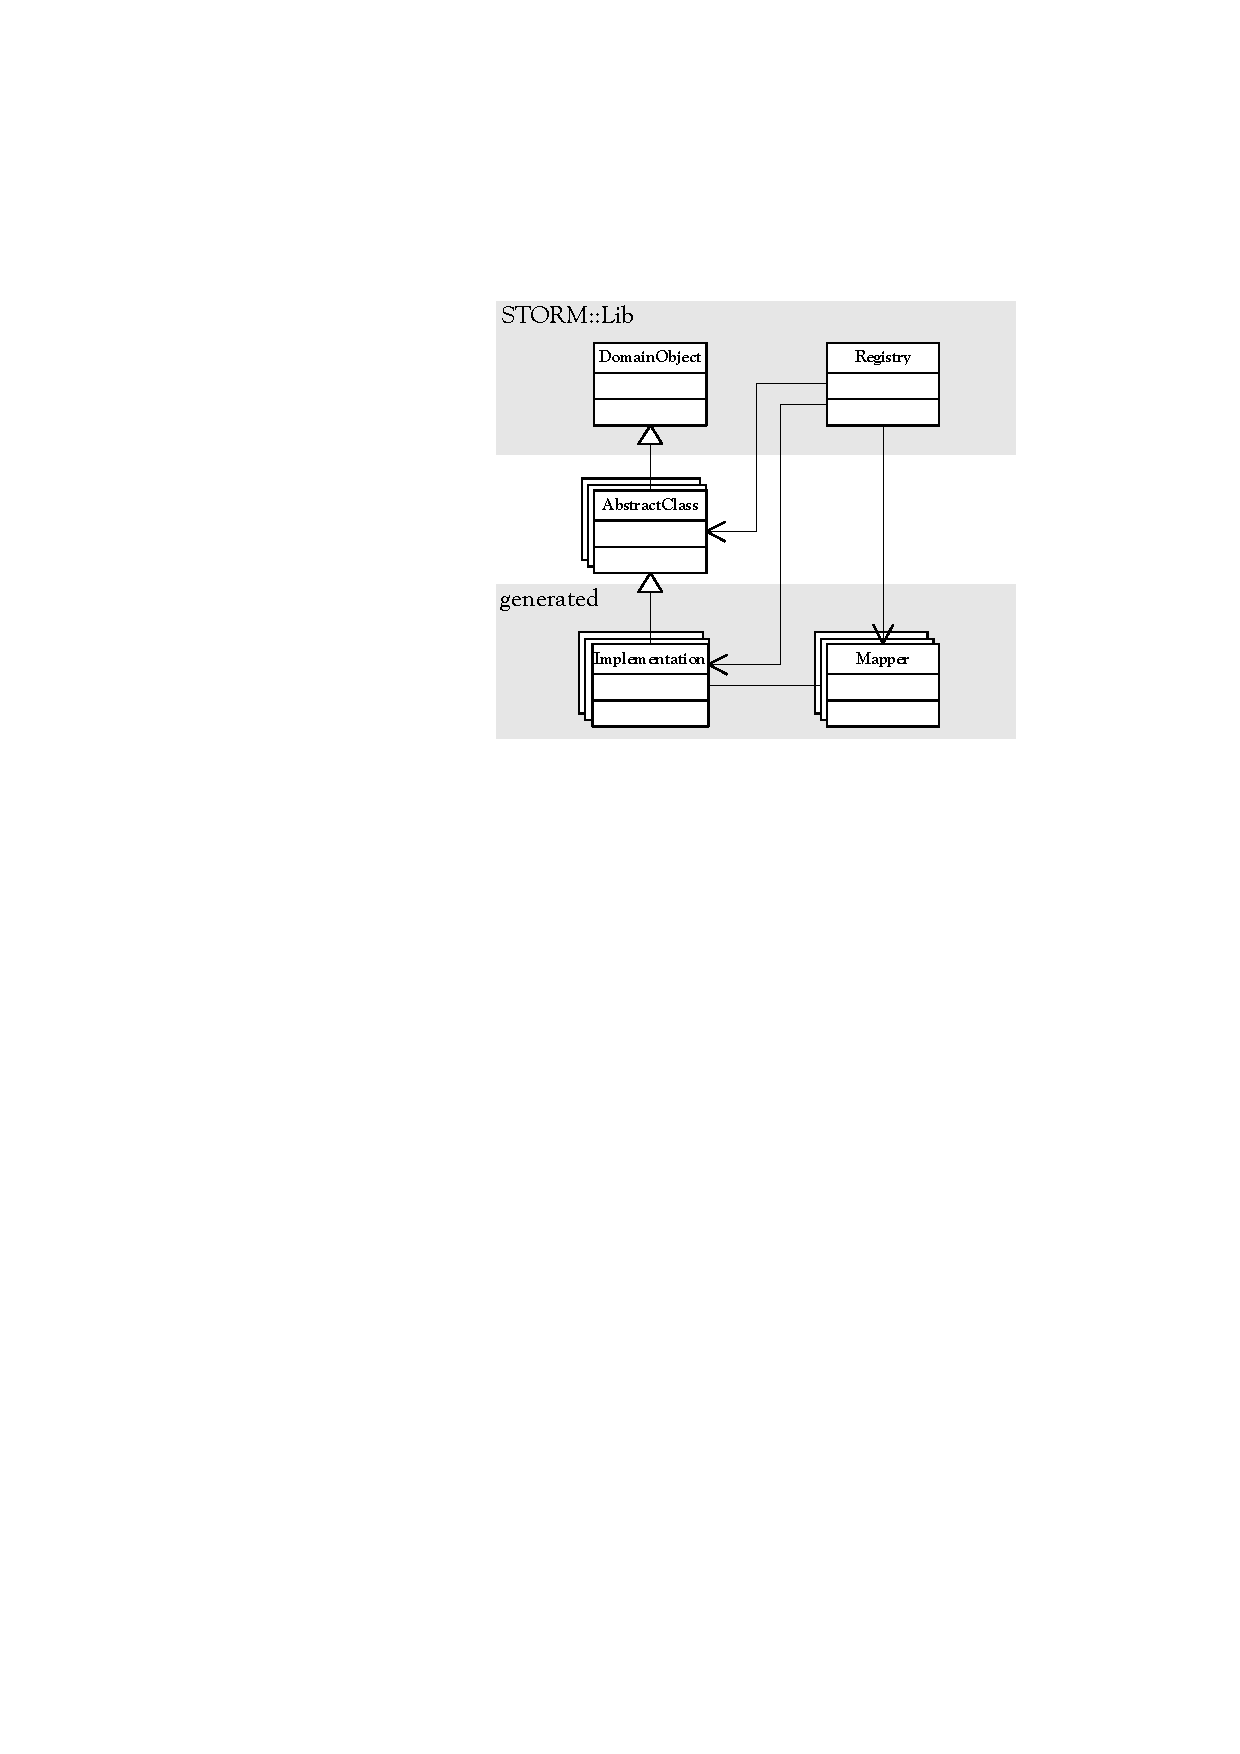
\includegraphics{./files/inc/figures/AnalysisKonzept1}
				\caption{\label{fig:AnalysisKonzept1} Vererbungsstruktur mit STORM}
			\end{center}
		\end{figure}
		
		Die Abbildung \ref{fig:AnalysisKonzept1} zeigt die Vererbungsstruktur vom einem \verb~DomainObject~ bis zur generierten 
		Implementation.
	
		Ein Problem, das gel�st werden muss, ist das Arbeiten mit den generierten Implementationen. Weder aus dem 
		selber geschriebenen Code noch aus anderen generierten Klassen, darf auf generierte Klassen 
		zugegriffen werden. Denn der Code muss auch kompilierbar sein, wenn noch kein oder nur ein Teil des Codes 
		generiert wurde.
		
		Damit jedoch der generierte Code auch genutzt werden kann, muss dieser an einer zentralen Stelle verwaltet werden.
		Hier kommt die Registry zum Einsatz.
				
	\section{Registry}
		
		Die generierten Klassen werden mit Attributen versehen. Wenn die Applikation gestartet wird, muss eine 
		Init Funktion der Registry aufgerufen werden, die den gesamten Code per Reflection analysiert und die 
		Implementationen der Domain Objekte sowie die dazugeh�rigen Mapper sucht und in einer Tabelle ablegt.
		
		Die nachfolgend beschriebenen Factory und Finder Klassen k�nnen von der Registry �ber ein statisches 
		Attribut in der Implementation geholt werden.
		
	\section{Factory}
	\label{sec:analyseFactory}
		Soll zum Beispiel ein Objekt der Implementation \verb~PersonImpl~ erstellt werden, muss zuerst von der Registry 
		mit dem abstrakten Typ \verb~Person~ dessen Factory geholt werden. Wie in Abbildung \ref{fig:AnalysisKonzept2} 
		gezeigt, ist die Factory eine interne Klasse der Implementation. Sie kann somit den Implementations Code 
		instanzieren, da er auf jeden Fall existiert. 
		
		Die generierte Factory stellt Standard Methoden zur Verf�gung. Diese werden aus dem selber geschriebenen Code    
		�ber das Interface IFactory aufgerufen.
		
		In der abstrakten Klasse k�nnen bei Bedarf zus�tzliche Factory Methoden beschrieben werden, die im generierten 
		Code implementiert werden. Die Beschreibung geschieht mit Attributen.
		
		\begin{figure}[hbt]
			\begin{center}
				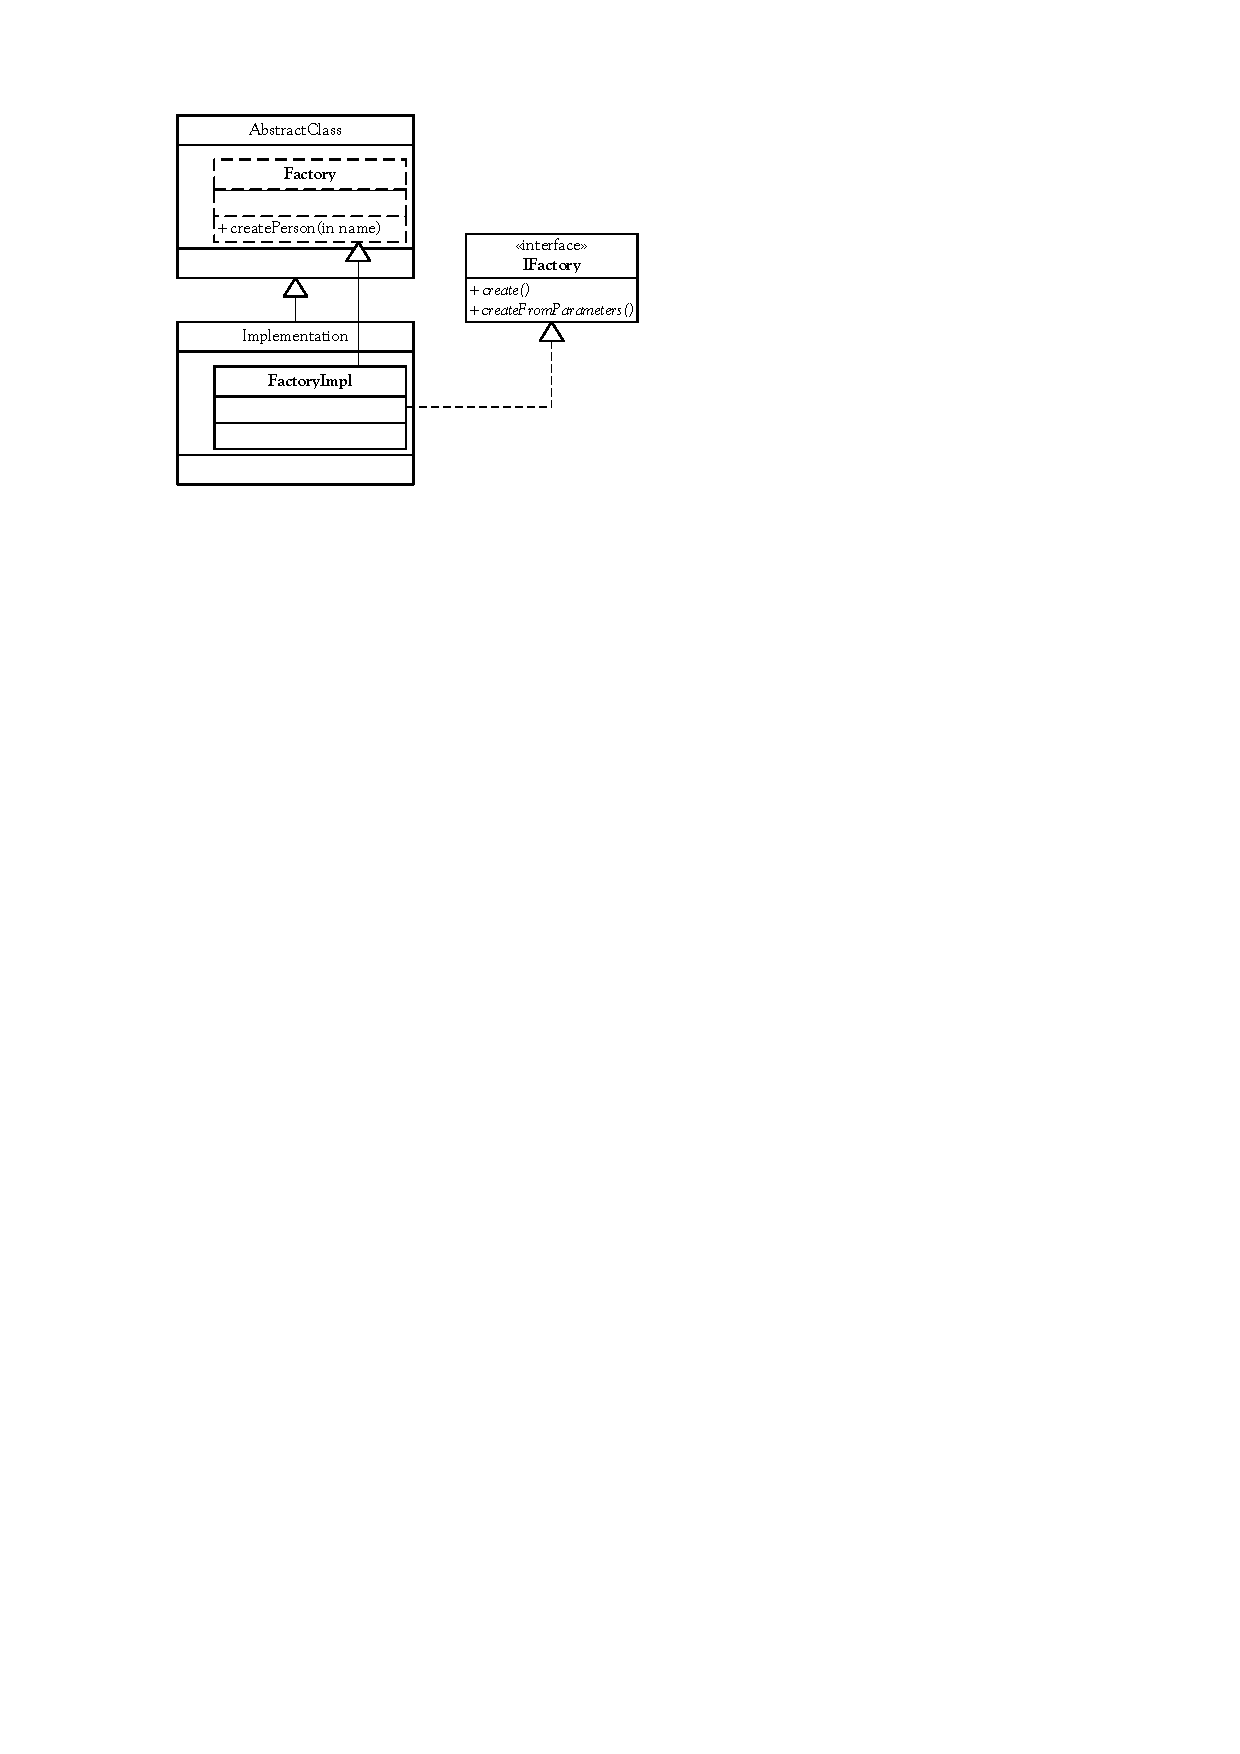
\includegraphics{./files/inc/figures/AnalysisKonzept2}
				\caption{\label{fig:AnalysisKonzept2} Business Objekt mit interner Factory Klasse}
			\end{center}
		\end{figure}
	
		
	\section{Finder}
	\label{sec:analyseFinder}
		Will man ein Objekt in der Datenbank suchen, muss man auf sogenannte Finder Methoden zugreifen k�nnen. Da diese
		Funktionen generiert werden, stehen wir vor dem gleichen Problem wie bei der Factory. Wie man in Abbildung
		\ref{fig:AnalysisKonzept3} sehen kann, werden die Finder Klassen ebenfalls als interne Klassen realisiert. 
		Die drei Standard Finder Methoden k�nnen �ber das Interface IFinder aufgerufen werden.
		
		In der abstrakten Klasse k�nnen wie bei der Factory zus�tzliche Finder Methoden beschrieben werden.
						
		\begin{figure}[hbt]
			\begin{center}
				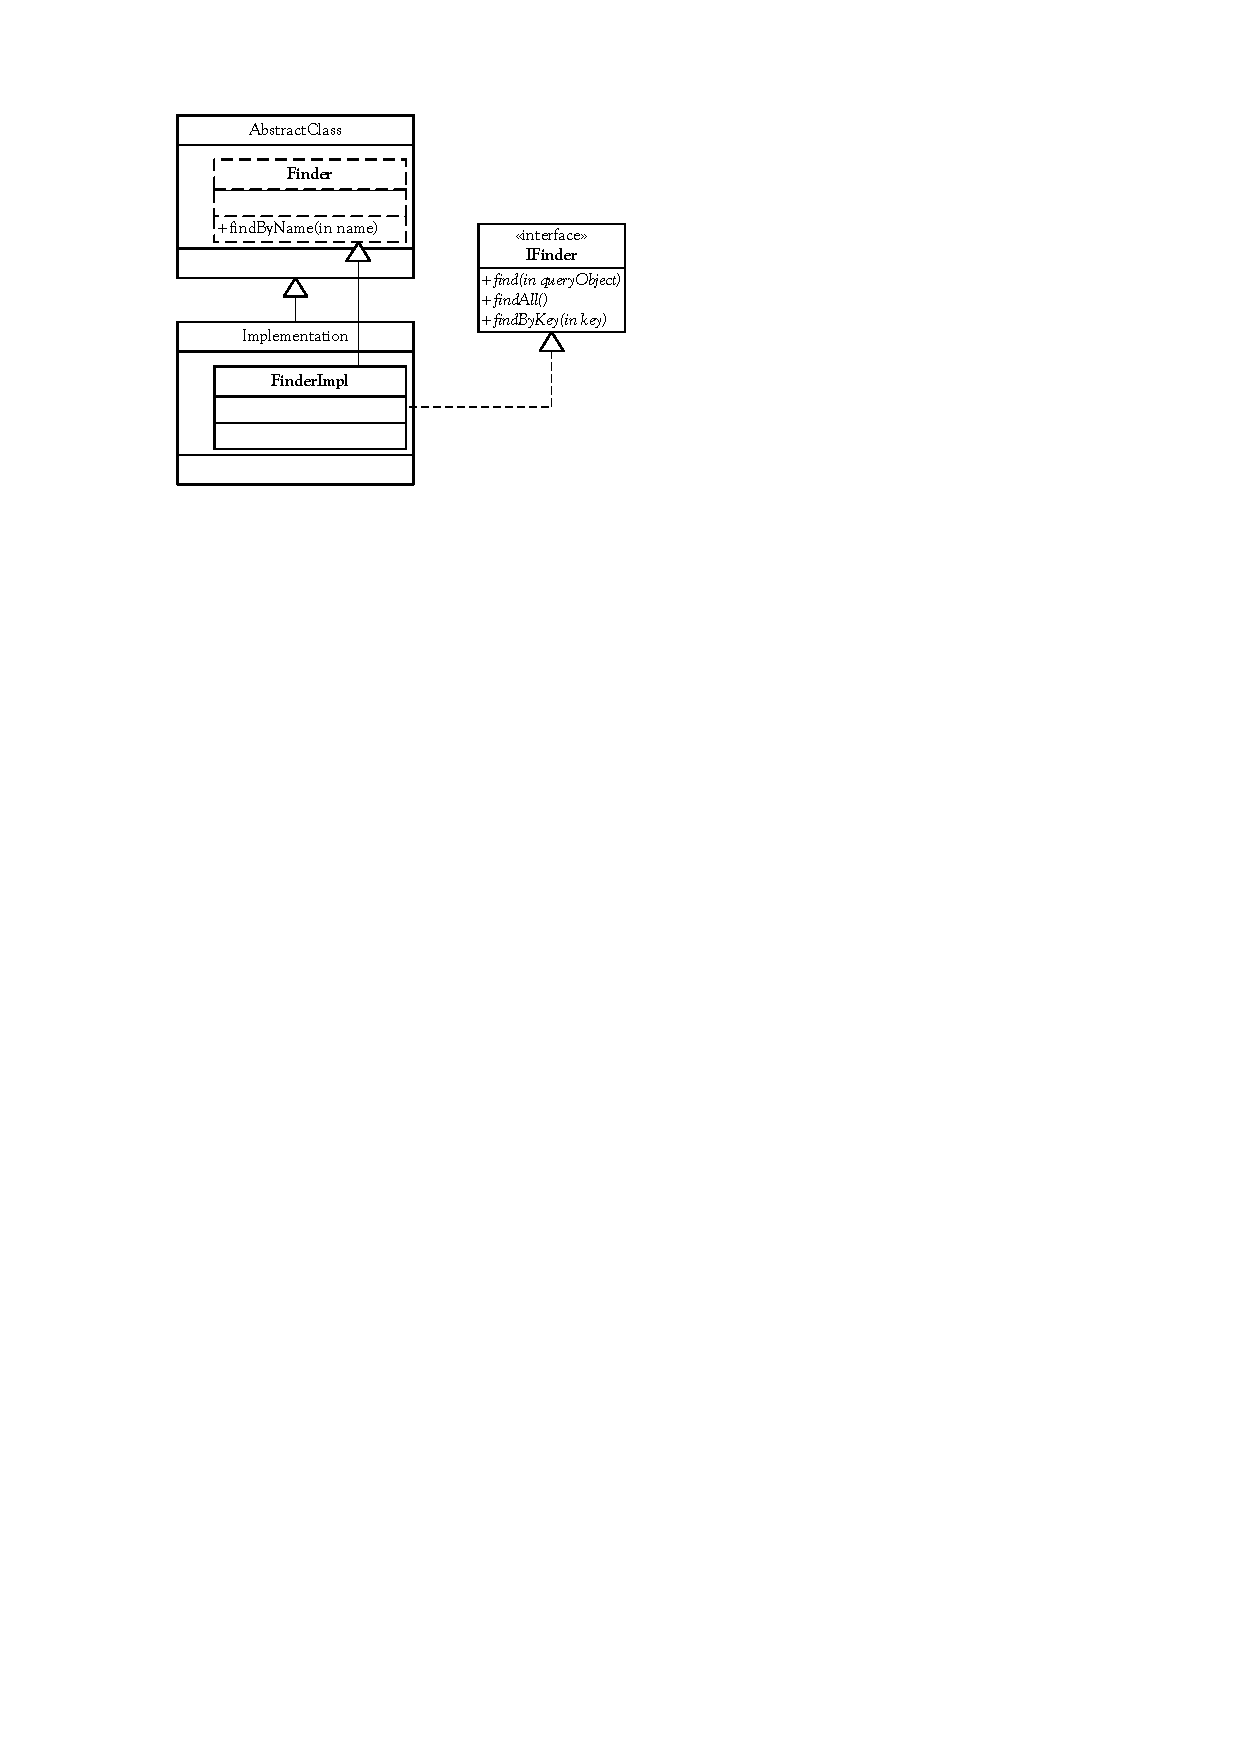
\includegraphics{./files/inc/figures/AnalysisKonzept3}
				\caption{\label{fig:AnalysisKonzept3} Business Objekt mit interner Finder Klasse}
			\end{center}
		\end{figure}
	
		Die Methode \verb~findAll()~ gibt eine Liste mit allen Objekten von einem bestimmten Typ zur�ck. \verb~findByKey()~
		sucht ein Objekt mit dem gew�nschten eindeutigen Schl�ssel. Der Methode \verb~find()~ kann ein QueryObject mitgegeben 
		werden, das Bedingungen f�r die Suche auf der Datenbanken speichert.
		
	\section{HsrOrderApp\_S4}
	
		Das Design der HsrOrderApp\_S4 wird vor allem durch die existierende Datenbank vorgegeben. 
		Das Modell der HsrOrderApp\_S3 wird wo m�glich �ber\-nommen. Eine der markantesten �nderungen 
		ist, dass die Domain Objekte in abstrakte Klassen und generierte Implementationen davon aufgeteilt 
		werden. Diese sind im konzeptionellen Modell auf der n�chsten Seite rot (abstrakt) und gr�n (generiert).
		
		Da sowieso alle Domain Objekte von der Oberklasse \verb~DomainObject~ abgeleitet werden m�ssen, 
		haben wir entschieden den Primary Key (Klasse \verb~Key~) und das Versions Feld (Klasse 
		\verb~Timestamp~) in die DomainObject Klasse auszulagern anstatt in die Implementationen zu generieren.
		Dies ist auch eine Erleichterung f�r den Programmierer, da er sie nicht in den abstrakten Klassen
		auff�hren muss.
		
		Das konzeptionelle Modell auf der n�chsten Seite zeigt bei den Domain Objekten die internen Factory 
		und Finder Klassen. Diese sind in den Abschnitten \ref{sec:analyseFactory} und \ref{sec:analyseFinder} 
		beschrieben.
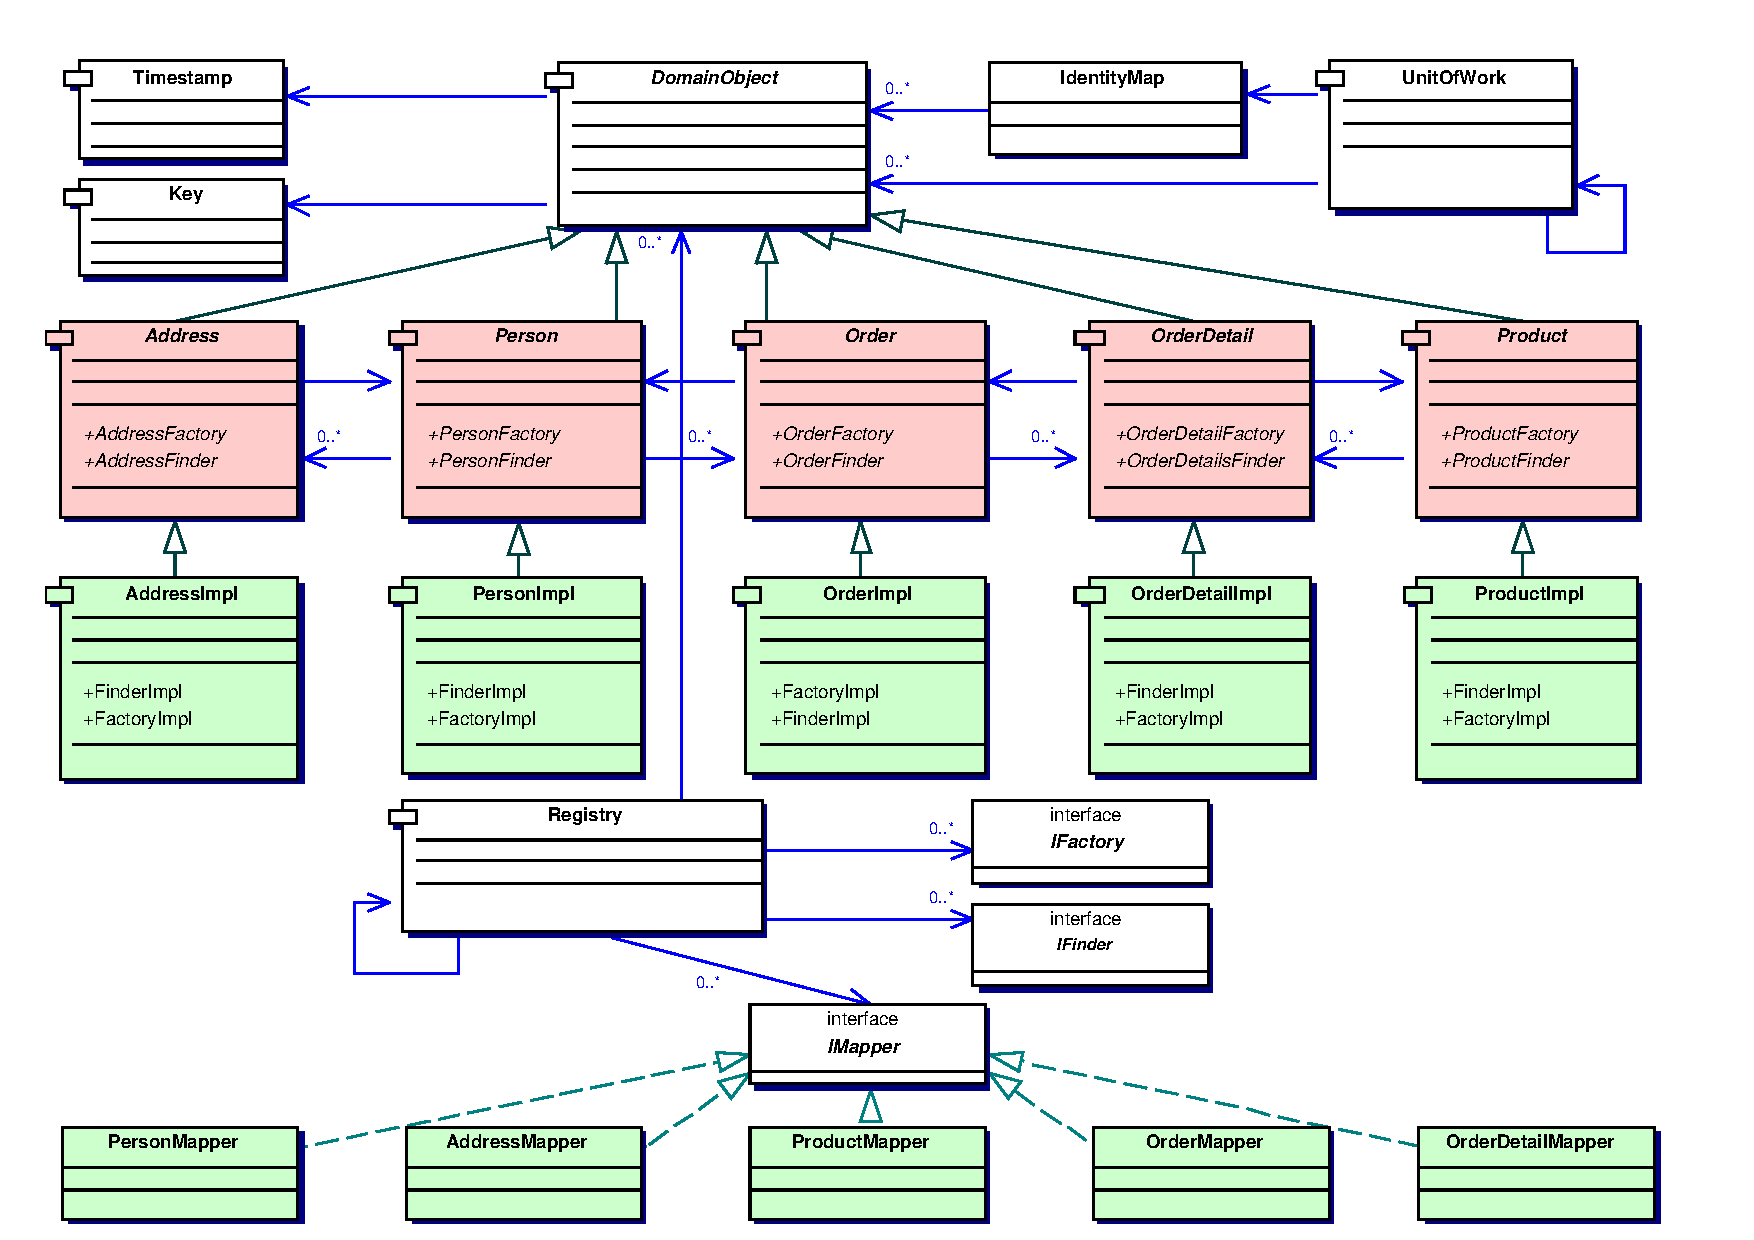
\includepdf[pages={1},landscape]{./files/inc/figures/AnalyseKonzeptionellesModell}
